\section{Inverted Indices}

\subsection{Implementation}
Based on the prototype for the project we implemented two inverted indexes. The InvertedIndexHashMap and InvertedIndexTreeMap are two subclasses of the superclass InvertedIndex which in turn implements the Index interface. The inverted index is a clever implementation of the SimpleIndex class trying to overcome the problems given by this naive implementation which for every query given looks through every website in the database. The purpose of an inverted index is to preemptively create an index of websites to word when the program is build, rather than performing the task at every query. In this scenario when a user makes a query the search will be performed on a Map object which maps words contained in the websites, to the website objects. In this way we increase the time needed for building the application, but we decrease the time needed for every single query. This results in an overall improvement of the performance.

The two subclasses have only one difference, they instantiate two different dynamic types of the map object. A Map is an interface which once implemented by a class will map a key to a value. The key needs to be unique but the value can be repeated.
The InvertedIndexHashMap inherits all the methods and variables from the abstract superclass InvertedIndex and instantiate a HashMap. The HashMap is an implementation of the Map interface, it maps a data value (in this case a Collection<Website>) to a specific key (in this case a string which represents one word present in a specific Website). The HashMap does not follow any index and the order of the objects contained can change over time.
On the other hand we have the InvertedIndexTreeMap, which instantiate a TreeMap dynamic type for the map variable and inherits all the methods and variables from the abstract superclass InvertedIndex. The TreeMap follows the same behaviour as the HashMap with only one important difference, the TreeMap has an ordered index of its mappings. The TreeMap is sorted following the natural order of the keys or according to a provided Comparator. In our case this means that the String key will be sorted alphabetically.

As said previously mentioned these two classes extend the superclass InvertedIndex which is an abstract class, this means that is not possible to instantiate an InvertedIndex object directly. This structure allows us to write the code in a more structured way, avoiding duplicate code and leading to easy extensibility of the application. Hence, we implement all the common behaviour of an index into the InvertedIndex superclass and then we implement the details into the specific subclasses.

Is this relevant?
When we create an object using a subclass as dynamic type, the constructor of the subclass will initialize the map object respectively as a HashMap or a TreeMap. Then when a method is called on the object, the compiler will perform a method-lookup, which means that it will look for the method in the subclass. But in this case it will find only the constructor, then it will look into the superclass that contain the build method and the lookup method. These two methods will perform their operations on the map object which was initialized into the sub-class constructor, so we use a TreeMap or a HashMap depending on the dynamic type declared at the object creation.


\begin{figure}[t]
	\centering
	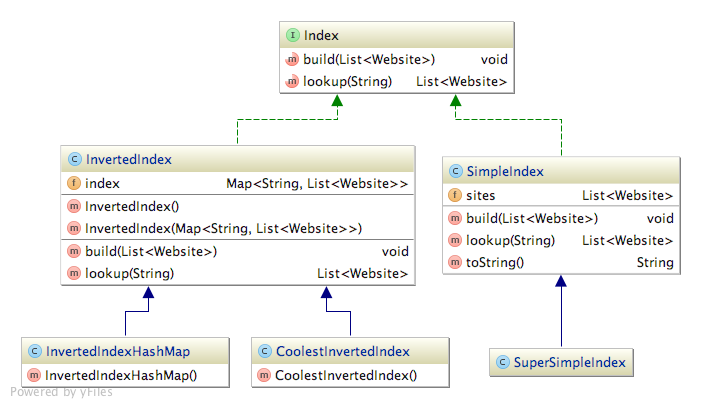
\includegraphics[width=\textwidth]{graphics/diagram-index.png}
	\caption{UML Diagram for the Software Architecture of Index data structures.}
	\label{fig:index:uml}
\end{figure}



\subsection{Benchmarking}
The different implementations are to be benchmarked and compared, the expected findings were that the TreeMap would outperform the HashMap implementation due to TreeMaps logarithmic growth of time cost of the .get method based on the map size, compared to the constant growth of time cost in the HashMap. 
The efficiency of the two indices is then expected to intersect at some map size, with HashMap being the most efficient up until a certain map size and TreeMap being efficient of sizes bigger than that.
The benchmark process was carried out multiple times in an attempt to reduce the error size of the process. This was to some extent possible although the error did not become entirely neglectable.
The results of the benchmarking can be found in appendix A.

Analysis and discussion:
The results of the benchmarking did not align completely with the result that was expected, the TreeMap implementation did not manage to outperform HashMap, evidently due to the limited size of the datafiles. 

\begin{table}[t]
\begin{tabular}{@{}llr@{}r} \toprule
	Index & File & Avg. lookup time (ms) &Error \\ \midrule
	SimpleIndex  & enwiki-tiny.txt	& -- & -- \\ 
				 & enwiki-small.txt	& -- & -- \\
				 & enwiki-medium.txt& -- & -- \\
	InvertedIndexTreeMap	& enwiki-tiny.txt	& -- & --\\
							& enwiki-small.txt	& -- & --\\
							& enwiki-medium.txt & -- & --\\
	InvertedIndexHashMap	& enwiki-tiny.txt	& -- & --\\
							& enwiki-small.txt	& -- & --\\
							& enwiki-medium.txt & -- & --\\ \bottomrule
\end{tabular}
	\caption{Running times for different index implementations.}
\label{tab:benchmark:indices}
\end{table}


